\documentclass[12pt]{article}

\usepackage[english]{babel}
\usepackage[utf8x]{inputenc}
\usepackage{amsmath}
\usepackage{graphicx}
\usepackage[colorinlistoftodos]{todonotes}
\usepackage{listings}
\usepackage{glossaries}
\usepackage{placeins}
\usepackage{fixltx2e}
\usepackage{scrpage2}
\usepackage{scrtime}

\clearscrheadfoot
\pagestyle{scrheadings}
\usepackage[
top    = 2.5cm,
bottom = 3cm,
left   = 3cm,
right  = 3cm]{geometry}
\setcounter{secnumdepth}{4}

\author{RoboNav}
\date{\today}


\begin{document}


\begin{titlepage}
\begin{center}
% Oberer Teil der Titelseite:

%NEEDS TO BE OUT COMMENTED sometimes
%\includegraphics[width=1.0\textwidth]{../../pictures/robonavlogo}\\  

\includegraphics[width=0.5\textwidth]{logo}\\  

\LARGE TGM - HTBLuVA Wien XX \\ Ballkomite  \\[1.5cm]

% Title
\rule{1.0\textwidth}{1mm}
{ \huge \bfseries \\[0.4cm]  \huge 2.Ballbesprechung \\ \LARGE HS1 \\[0.4cm] }

\rule{1.0\textwidth}{1mm}



\noindent 
\vspace{6cm}
\small
\begin{center}
  \begin{tabular}{ | p{0.1\textwidth} | p{0.2\textwidth} | p{0.12\textwidth} | p{0.1\textwidth} | p{0.3\textwidth} |}
    \hline
\textbf{Version} & \textbf{Author} & \textbf{Date} & \textbf{Status} & \textbf{Comment} \\ 
    \hline 
    \hline
0.1 & Hannah Siegel & 2014.12.02 & Draft &    \\ 
0.2 & Hannah Siegel & 2014.12.03 & Draft &    \\ 
0.3 & Hannah Siegel & 2014.12.04 & Finished & Ready for Meeting    \\ 

    \hline
  \end{tabular}
\end{center}

\vfill

% Bottom of the page
{\small Version: \today ~at  \thistime    }
\end{center}

%\end{center}
\end{titlepage}
\tableofcontents





%HEADER AND FOOTER
\pagenumbering{arabic}
\ifoot{© Hannah Siegel}
\ofoot{\pagemark }

\section{Anwesenheit}
  \begin{tabular}{ | p{0.3\textwidth} | p{0.1\textwidth} |  p{0.1\textwidth} |}
    \hline
\textbf{Person} & \textbf{1.} & \textbf{2.}  \\ 
    \hline 
    \hline
 
Hannah Siegel & x & x\\ \hline
Arian LongHouse & x & E \\ \hline
Philipp Vogt & x & x\\ \hline
Janusz Gradonski & x & \\ \hline
Daniel Melichar & x &x \\ \hline
Dominik Scholz & E & x\\ \hline
Florian Brandstetter & x & L \\ \hline
Nadja Smolnig & x & x\\ \hline
Isabella Krammer & x & L \\ \hline
Nadja Hauer & x & x \\ \hline
Tatjana Gajic & x & x\\ \hline
Philip Orosz & x & E \\ \hline
Astrid Krickl & E & x \\ \hline
Richard Bauer & x & x \\ \hline
Julia Eichberger & & x\\ \hline
Bettina Nedwed & x & L\\ \hline
Julia Brandl & x & x\\ \hline
Wolfgang Biegel  & x &x \\ \hline
Vennesa Belinić & x &x \\ \hline
  \end{tabular}
  E ... Entschuldigt \\
  L ... Lernen
\newpage
\section{Hannah traegt vor:}
\subsection{Hardfacts - Wiederholung}
Ball am 20. Februar \\
Einlass 20 Uhr, Eroeffnung 21 Uhr
\subsection{Besichtigung Palais Auersperg}
Wahrscheinlich naechste Woche Freitag.
\subsection{DJs}
Diese werden von uns Ausgesucht (ca. 2) \\
Kevin Polley \\
Arian LongHouse (eigentlich fix am Start) 
\subsection{Fotografen}
Wird von Herbststrasse geklaert, faellt nicht unter unseren Taetigkeitsbereich.
\subsection{Crash Kurs}
Beim Crash-kurs werden ein paar wirklich einfache Grundsaetze gelernt.
\\
Dieser ist gratis und wird bei der Herbststrasse stattfinden. Wir suchen ganz besonders Burschen hierfuer. \\
Mittwoch, 28.1.2015 - 14 bis 15 Uhr \\ 
Mittwoch, 04.2.2015 - 14 bis 15 Uhr \\ 
Mittwoch, 11.2.2015 - 14 bis 15 Uhr \\
Donnerstag, 18.2.2015 - 14 bis 15 Uhr 
\subsection{Eintaenzen}
\subsubsection{Tanzschule}
Tanzschule Elmayer, Macht auch Mitternachtsquadrille
\subsubsection{Termine der Proben}
Mittwoch, 11.2.2015 - 17 bis 19 Uhr \\ 
Donnerstag, 12.2.2015 - 17 bis 19 Uhr \\
Donnerstag, 19.2.2015 - 17 bis 19 Uhr \\
Generalprobe am 20.2.2015 im Ballsaal ab 18 Uhr
\subsubsection{Anmeldung zum Eintanzen}
\textbf{Ausnahmslos} ueber Formulare.
\subsection{Plakat}
\begin{figure}[here!]
\centering
\begin{minipage}[h]{0.25\textwidth}
\centering
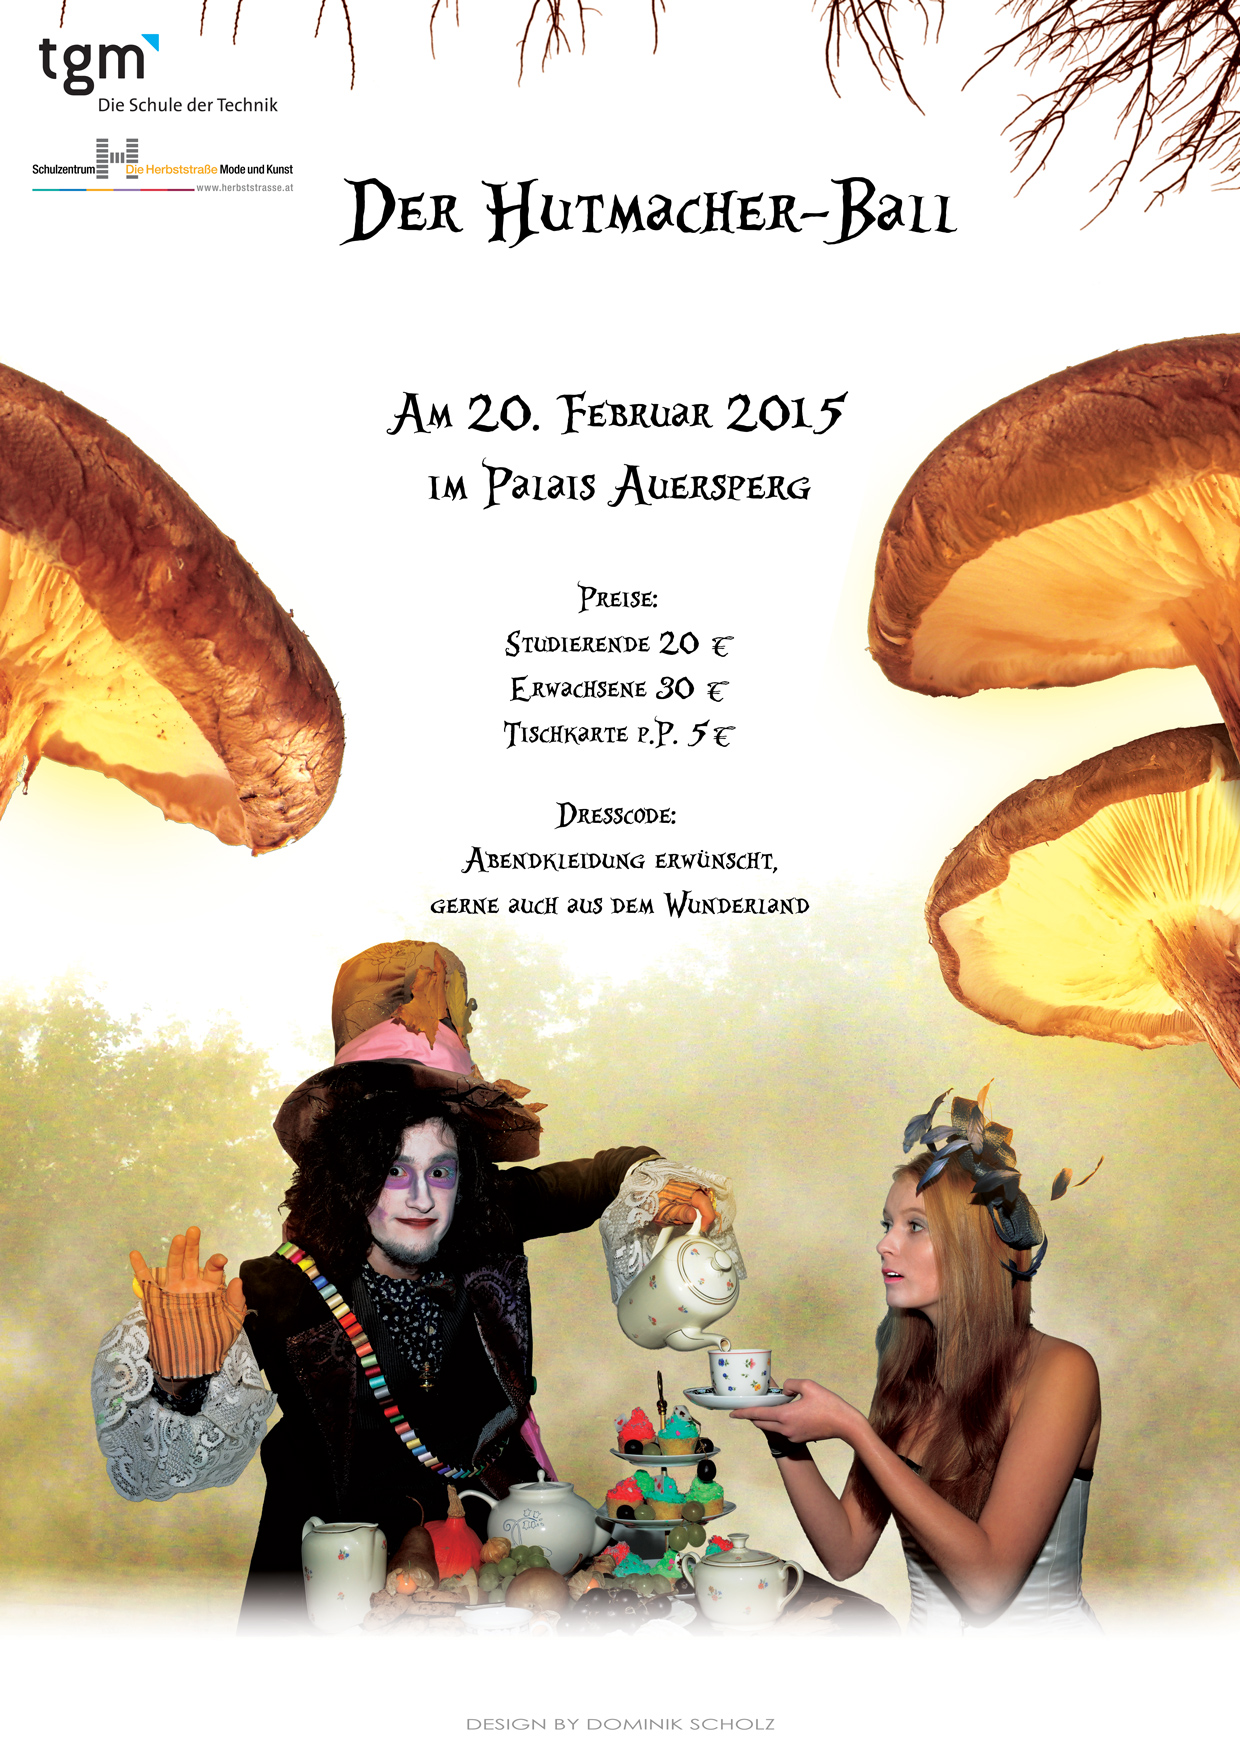
\includegraphics[width=1.0\textwidth]{versionbright_small}
    \caption{Finaler Entwurf}
    \label{fig:eai0}
\end{minipage}
\begin{minipage}[h]{0.25\textwidth}
\centering
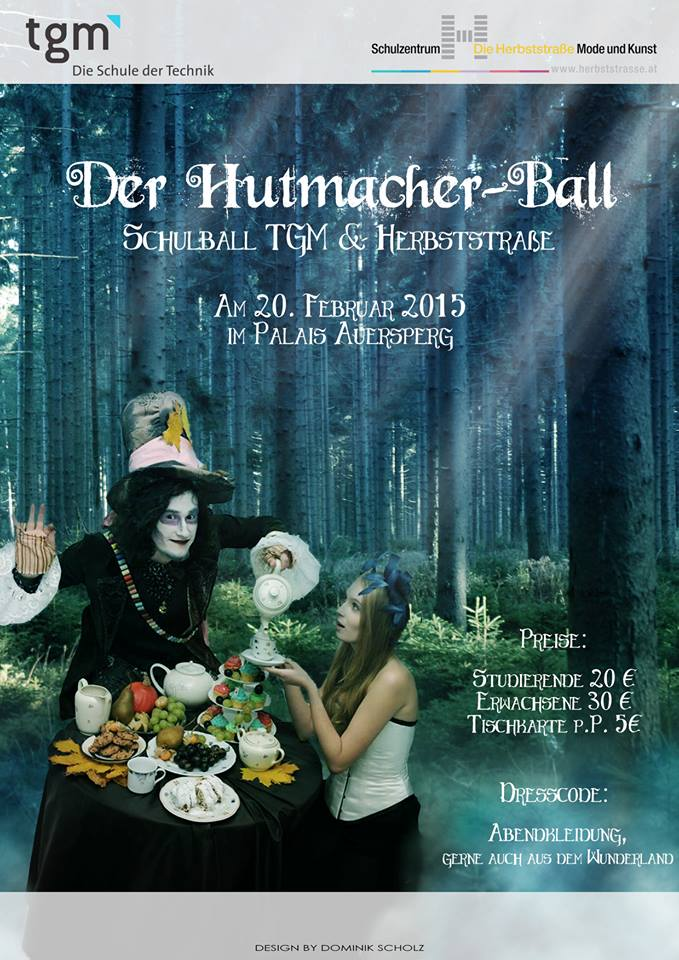
\includegraphics[width=1.0\textwidth]{fertig} 
    \caption{Zweiter Entwurf, gilt nur fuer Herbststrasse}
    \label{fig:eai1}
\end{minipage}
\end{figure}
\subsection{Eintrittskarten}
\subsubsection{Kartenverkauf}
Ab \textbf{ 15.Dezember} beim  Verband der TechnologInnen (1.Stock) \\
Eventuell Ausnahmen fuer Abendschueler. \\ \\
Ermaessigt: 20 Euro \\
Normal: 30 Euro
\subsubsection{Gratis Eintritte}
Ihr bekommt, der Regel nach, KEINE Karten.
\begin{enumerate}
\item Eintaenzer gratis Eintritt (Sind frueher da)
\item Schulballkomite gratis (bei Anwesenheit!) (Sind frueher da, stehen auch auf der Liste)
\item Mitternachtseinlagenteilnehmer gratis (betrifft nur Herbststrasse)
\item DJs und Aehnliche gratis (Sind frueher da)
\item AS \& SV vorraussichtlich nicht gratis 
\end{enumerate}
\subsubsection{Tischkarten}
5 Euro pro Person, Verkauf beim Verband der TechnologInnen. \\
Wenn Tische ueber bleiben, bekommt das Ballkomite/die Eintaenzer diese.

\subsection{Deko}
Schach, Poker \\
Stoffe beim Eingang \\
Tischdeko \\
\subsubsection{Technische Deko}
\begin{enumerate}
\item Schulball App
\item Projektpresentation des Apps am Montag vor Weihnachten? Wer will kommen?
\item Polaroid Kameras beim Eingang - Personen werden abgestempelt
\end{enumerate}
\subsection{Ballkoeniging und Ballkoenig}
Wahl vorraussichtlich von dem BESTEN KOSTUEM!
\\
Wahl wahrscheinlich ueber die Schulball-App oder ueber Boxen, oder ueber Facebook oder ueber eine Jury.
Wahrscheinlich jeweils ein Gewinner des TGMs und ein Gewinner der Herbststrasse.
\newpage
\subsection{Organisation am Balltag}
\subsubsection{Meetings}
Es werden fixe Treffpunkte ausgemacht werden (am Balltag und waehrend des Balles)
\subsubsection{Handys}
Jeder sollte sein Handy mithaben bitte.
\subsubsection{Alkohol}
Ist erlaubt, aber wenn ihr Tasks (wie zum Beispiel Kipferl austeilen) habt, bitte \textit{halbwegs} nuechtern :)
\subsubsection{Zeitplan fuer den Balltag}
Ein genauer Zeitplan fuer den Balltag wird beim 3.Ballkomitee treffen presentiert.
\subsubsection{Kontaktinformationen}

 \begin{tabular}{ | p{0.3\textwidth} | p{0.2\textwidth} |  p{0.5\textwidth} |}
    \hline
\textbf{Person} & \textbf{Klasse} & \textbf{Nummer}  \\ 
    \hline 
    \hline
   
Hannah Siegel & 5AHITT & \\ \hline
Arian LongHouse &  & \\ \hline
Philipp Vogt & 4BHBG & 0680 2162382 \\ \hline
Janusz Gradonski&  & \\ \hline
Daniel Melichar& 4CHITM & 0660 7124392 \\ \hline
Dominik Scholz & 5AHITT & 0676 6936944 \\ \hline
Florian Brandstetter &  3BHBG & 0660 4449933 \\ \hline
Nadja Smolnig & 5CHWIL & 0664 1806915 \\ \hline
Isabella Krammer & 3BHBG & 0699 13765300 \\ \hline
Nadja Hauer &  4BHBG & 0664 5432396 \\ \hline
Tatjana Gajic & 3BHEL & 0676 9059116 \\ \hline
Philip Orosz & 4CHIT & 0676 9056473\\ \hline
Astrid Krickl & 5BHITM & 0660 5525298 \\ \hline
Richard Bauer & 4AHETE & 0699 17176514 \\ \hline
Julia Eichberger & 4BHBG &  0660 1931997\\ \hline
Bettina Nedwed & 3BHBG & 0699 18229127 \\ \hline
Julia Brandl & 4BHBG & 0681 10346606\\ \hline
Wolfgang Biegel  & 3/4 ABEL & 0676 88680239\\ \hline
Vennesa Belinić & 5AHITT & 0664 4950701 \\ \hline
  \end{tabular}
\FloatBarrier
\newpage
\section{Input von euch:}
\begin{enumerate}
\item Ideen fuer Verwendung der QR codes?
\item Ideen fuer Umsetzung von Schach und Poker?
\item Brainstorming wegen Hueten der Eintaenzer / Special Dekoration
\item Ideen wegen Aftershow party?
\item Brainstorming wegen Raucherraum
\item hat irgendwer Wakey Talkies zuhause?
\end{enumerate}
Antworten: \\
Vennesa hat eventuell Walkey Talkeys \\
Weltkugel als Deko \\
Figuren die Herumgehen? \\
Musikwahl \\
Schach/Poker wird nicht umgesetzt \\
\\\textbf{zu den Eintanzern:} \\
Fascinators selbermachen? \\
Zylinder ausborgen? \\
Stylistin? \\ \\
\textbf{zu den QR codes:} \\
Als 'Partnersuche' \\
Muessen Ausgedruckt werden, von M1 und B1, ....  \\
Man bekommt Zuckerl zb wenn man das schafft \\
\\ 
Getraenkekarte\\
DJ-LineUP \\
Sind die QR codes ee offline zugaenglich \\
Aftershowparty gerne gesehen
\newpage
\section{Einteilung}
  \begin{tabular}{ | p{0.35\textwidth} | p{0.20\textwidth} |  p{0.5\textwidth} |}
    \hline
\textbf{Aufgabe} & \textbf{Datum / Uhrzeit} & \textbf{Personen / Veranntwortlichen} \\ 
    \hline 
    \hline
\textbf{Vorm Balltag} &  &  \\ 
  &  &  \\ \hline
DJs auswaehlen (4) & bis ende Dezember & Arian, Philipp V. \\ 
  &  &  Janusz , Philip O.\\ \hline
Organisation After show Party wenn gewollt (2) & bis Anfang Jaenner & Dominik, Astrid  \\ \hline
Organisation Crashkurs (1) & bis mitte Dezember &  Hannah, Nadja S\\ \hline
Organisation Wahl des besten Kostuemes (2) & bis mitte Jaenner &  Hannah, Nadja S \\ \hline
\textbf{Am Balltag} &  &  \\ 
  &  &  \\ \hline
Kipferl holen (2) & ca 14:00 & Bettina Nedwed, Isabella Krammer \\ \hline
Kipferl einpacken (4) & ca 15:00 & Bettina, Isabella \\ 
  &  & Hannah, Tatjana  \\ \hline
Kipferl austeilen Schicht 1 (2) & von 0:30 bis 1:30 & Vennesa, Julia E.  \\ \hline
Kipferl austeilen Schicht 2 (2) & von 1:30 bis ende & Nadja H, Julia B.  \\ \hline
Karten abreissen Schicht 1 (2) & von Anfang bis 22:00 & Daniel, Nadja S. \\ \hline
Karten abreissen Schicht 2 (2) & von 22:00 bis noetig &  Hannah, Julia E. \\ \hline
Deko helfen (4) & Ganzen Nachmittag & Nadja, Julia \\
  &  & Richard, Tatjana, Philipp \\ \hline
DJs Aufbauen helfen (1) & ca 19:00 & Philipp \\ \hline
Beim Fotografen aufbauen helfen (2) & ca 17:00 & Astrid, Julia E. \\ \hline
Eintaenzer organisieren (1) &  ca 18:00 & Wolfgang \\ \hline
Mitternachtseinlage helfen (1) & ca 22:00 & Tatjana \\ \hline
Auszaehlen Wahl des besten Kostuemes (6) & kurz vor 24:00 & Flo, Isabella  \\ 
  &  & Betti, Daniel  \\ 
  &  & Hannah, Richard \\ \hline
\textbf{ALLE} &  &  \\ 
  &  &  \\ \hline
Vorm Eintanzen den Ballsaal fuellen, platz machen &  & Alle  \\ \hline
Durchgehen und kontrollieren ob alles passt &  & Alle  \\ \hline
Durch die Klassen gehen und die Informationen verteilen & bis 15. Dezember &  Alle\\ \hline
Plakate aufhaengen & mitte Dezember & Alle  \\ \hline

\hline
\end{tabular}
  
%Arian LongHouse 
%Philipp Vogt 
%Janusz Gradonski
%Daniel Melichar 
%Dominik Scholz
%Florian Brandstetter 
%Nadja Smolnig
%Isabella Krammer 
%Nadja Hauer 
%Tatjana Gajic 
%Philip Orosz
%Astrid Krickl 
%Richard Bauer 
%Julia Eichberger
%Bettina Nedwed
%Julia Brandl 
%Vennesa Belinić 
%Wolfgang Biegel
\subsection{Verantwortliche / Chefes}

\begin{tabular}{ | p{0.4\textwidth} | p{0.6\textwidth}  |}
    \hline
\textbf{Aufgabe} & \textbf{Verantwortliche}  \\ 
    \hline 
    \hline
  
DJs  & Arian LongHouse \& Janusz\\ \hline
Erste Hilfe & Hannah  \& Bettina \\ \hline
Securities  & Hannah  \& Lisa \\ \hline
Eintaenzer & Isabella  \& Wolfgang\\ \hline
Ballkomite &  Hannah  \& Lisa \\ \hline
Probleme &  Hannah  \& Lisa \\ \hline
  \end{tabular}

\subsection{Klasseneinteilung}
  \begin{tabular}{ | p{0.4\textwidth} | p{0.3\textwidth}  |}
    \hline
\textbf{Verantwortlicher} & \textbf{Abteilung}  \\ 
    \hline 
    \hline
 
Philipp Vogt & BM  \\ \hline
Daniel Melichar & IT  \\ \hline
Nadja Smolnig & WI \\ \hline
Nadja Hauer & KT   \\ \hline
Tatjana Gajic & EL  \\ \hline
Richard Bauer & ET \\ \hline
Julia Brandl & MI \\ \hline
Wolfgang Biegel  & AS (16 Klassen)\\ \hline
  \end{tabular}
  \subsection{Naechste Treffen}
  Wenn nicht anders Angegeben, dann in der Aula des 9. Stocks :) \\
  Andere kleinere (noetige) Besprechungen werden einfach spontan ausgemacht. \\
 \begin{tabular}{ | p{0.3\textwidth} | p{0.2\textwidth} |  p{0.5\textwidth} |}
    \hline
\textbf{Treffen} & \textbf{Termin} & \textbf{Personen}  \\ 
    \hline 
    \hline

DJs & 9.1 - 9:50 & mit DJs \\ \hline
After Show Party & 22.12 - 9:50 &  \\ \hline
After Show Party & 8.1 - 9:50 &  \\ \hline
After Show Party & 2.2 - 9:50 &  \\ \hline
Crashkurs & 16.12 - 9:50 &  \\ \hline
Austeilung Plakate & 12.12 - 9:50 & alle \\ \hline
Kipferl  & 20.02 - 9:50 &  \\ \hline
Karten  & 19.02 - 9:50 &  \\ \hline
SchulballApp  & 22.12 - ca 6.Stunde &  \\ \hline
'BallkoenigIn'  & 22.12 - 9:50 &  \\ \hline
'BallkoenigIn'   & 28.01 - 9:50 &  \\ \hline
\textbf{3 . Ballkomite treffen}   & 25.01 - 11.Stunde & alle - wsl HS1 \\ \hline
\textbf{4 . Ballkomite treffen}   & 12.02 - 11.Stunde & alle - wsl HS1 \\ \hline
\textbf{Balltag}  & \textbf{21.02 - 19:00} & \textbf{alle} \\ \hline


  \end{tabular}
  \newpage

\end{document}
